AERCA có thể khôi phục nhiều phụ thuộc liên quan, nhưng đồ thị thô thường dày hoặc chứa các liên kết khó diễn giải về mặt hành vi. Vì vậy, CausClass dùng LLM như một bộ sinh đề xuất trong quá trình tìm kiếm đồ thị. Về mặt phương pháp, LLM chỉ đóng vai trò đề xuất chỉnh sửa cấu trúc dựa trên mô tả biến, đồ thị hiện tại, phản hồi từ các lần thử trước và tín hiệu hệ số thô; nó không được quyết định đồ thị cuối cùng. Các lựa chọn mô hình cụ thể và cấu hình chạy được trình bày trong Chương 4.

\begin{figure}[htbp]
  \centering
  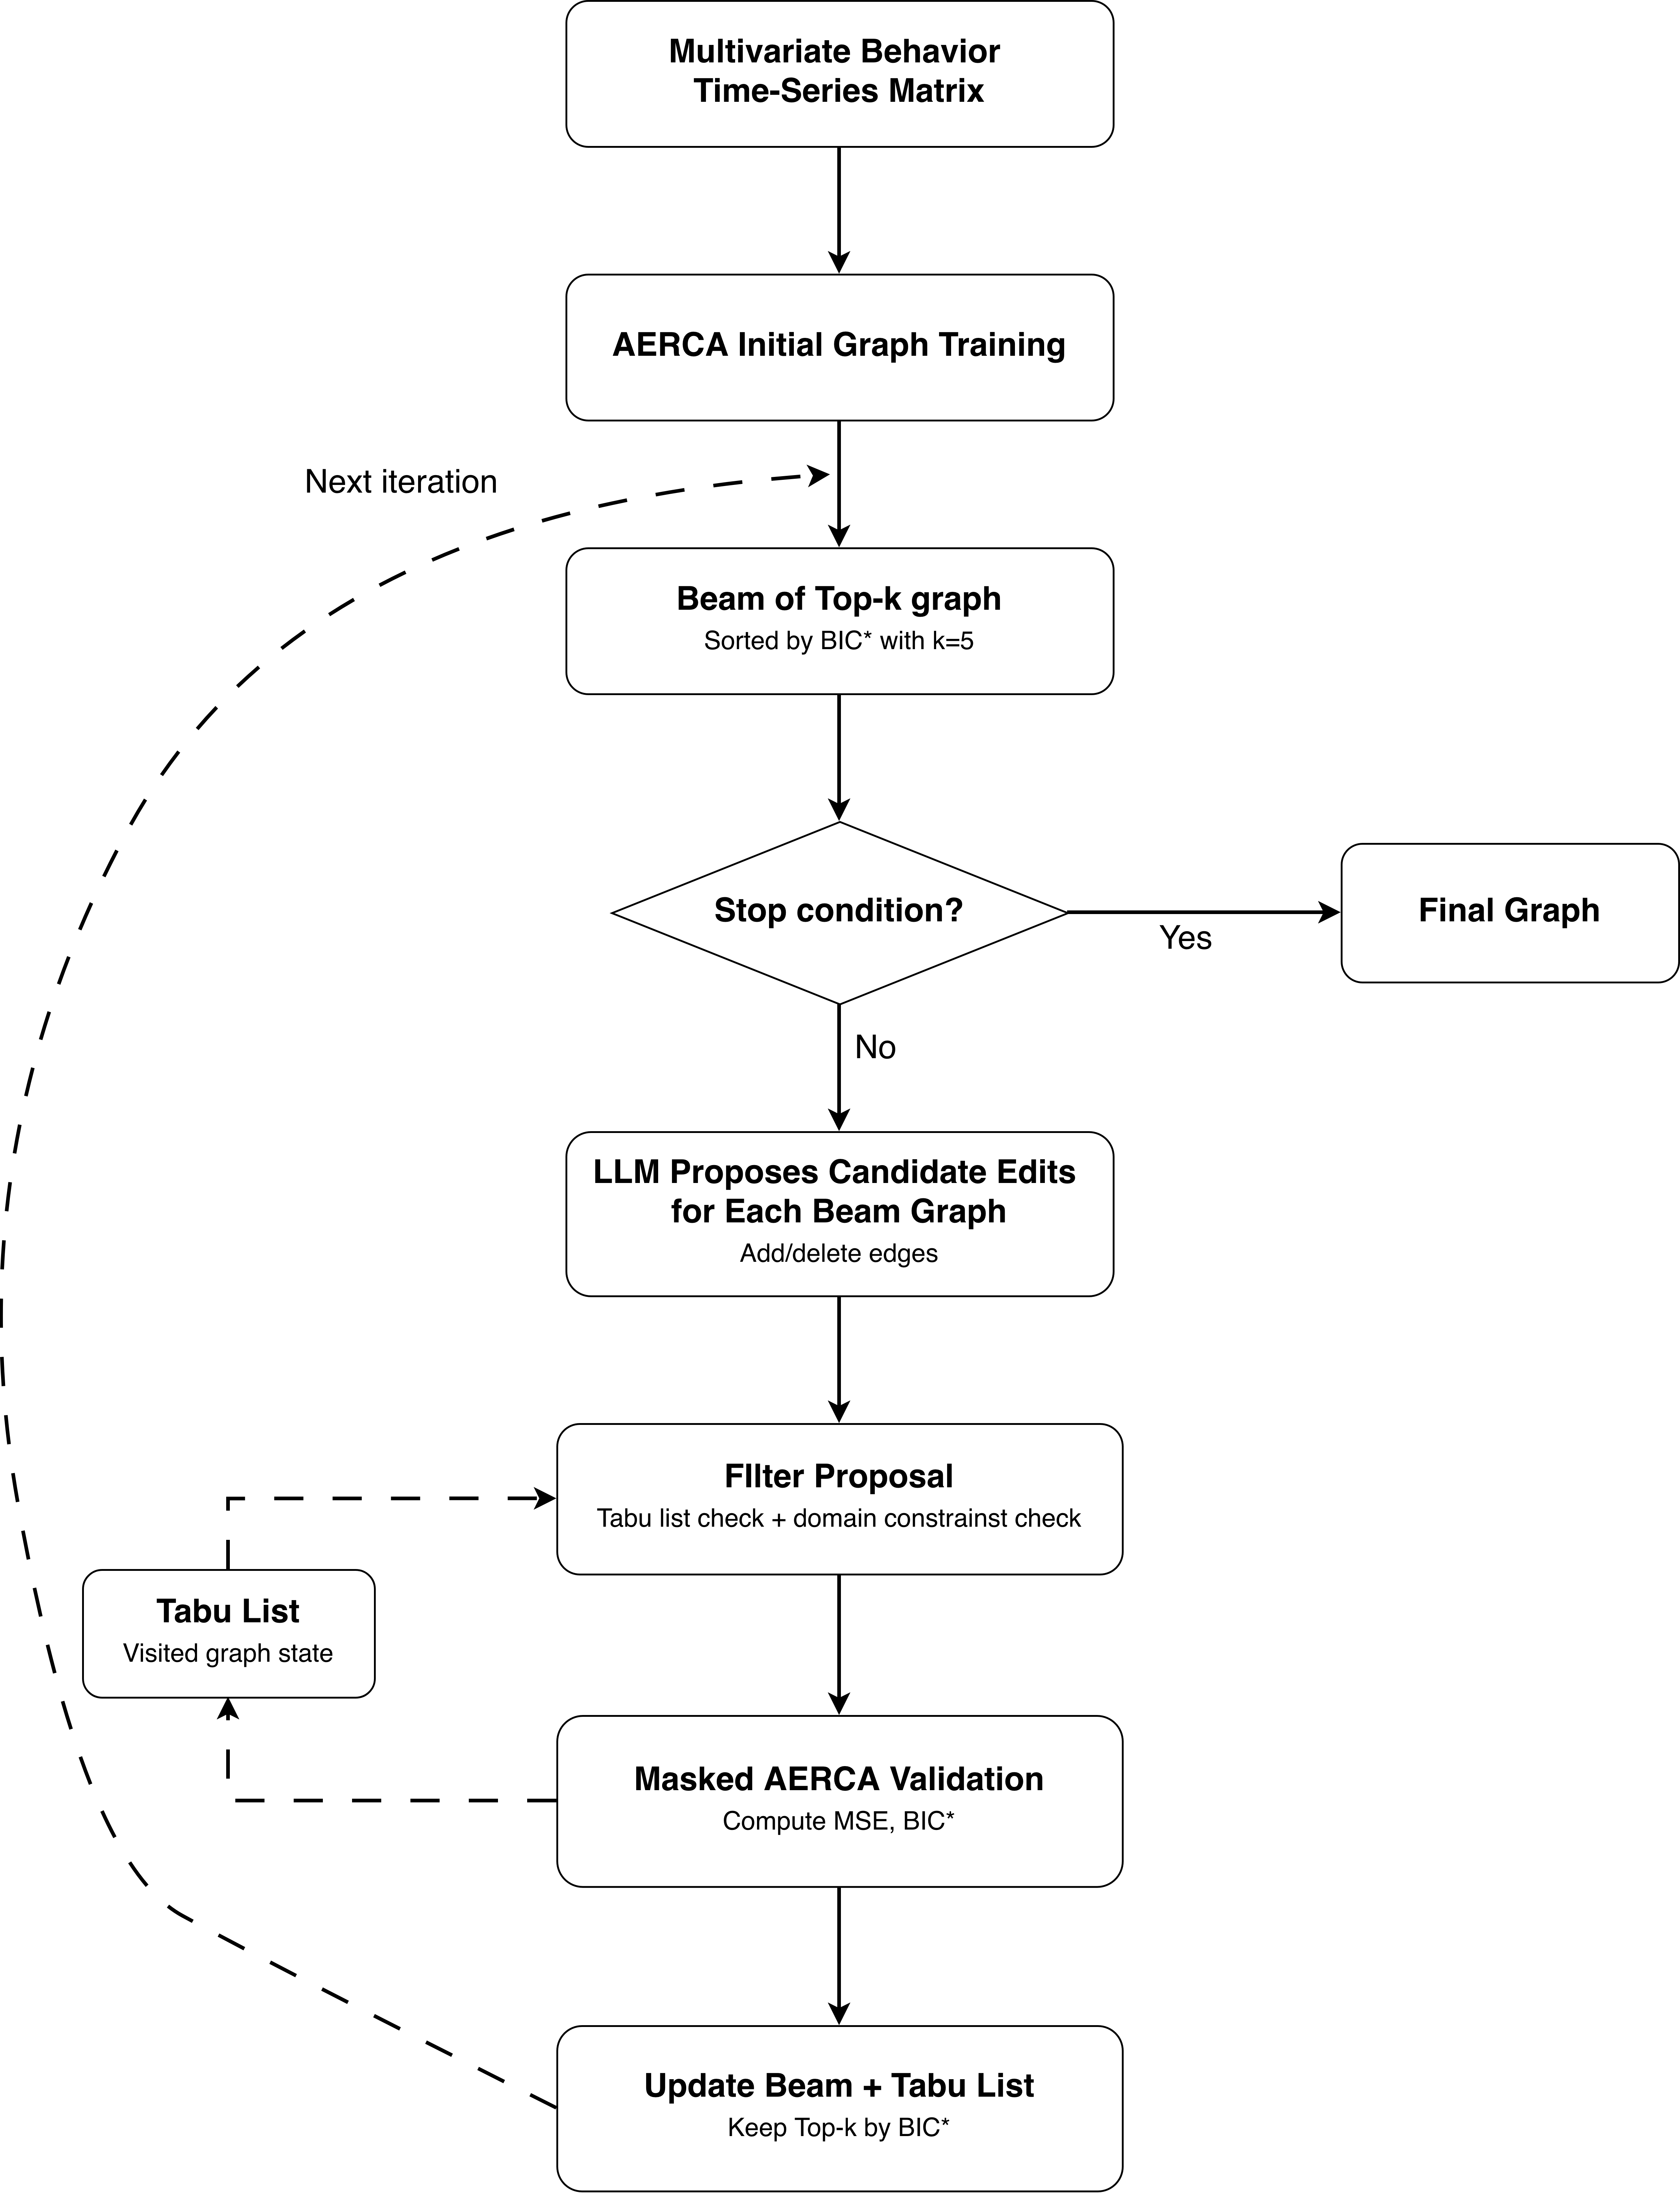
\includegraphics[width=0.95\textwidth]{figures/stage2.png}
  \caption{Pipeline chi tiết của Stage 2. AERCA tạo đồ thị khởi tạo và tín hiệu hệ số thô; LLM đề xuất thao tác thêm/xóa cạnh; masked AERCA kiểm chứng từng ứng viên; beam search giữ các đồ thị gọn có điểm validation tốt hơn.}
  \label{fig:stage2}
\end{figure}

Tại mỗi bước tìm kiếm, hệ thống biểu diễn đồ thị hiện tại thành danh sách cạnh và cung cấp cho LLM các ràng buộc miền cần tuân thủ. LLM sinh một tập nhỏ thao tác chỉnh sửa, chẳng hạn thêm hoặc xóa cạnh có hướng. Các thao tác này được lọc để loại bỏ chỉnh sửa không hợp lệ, trạng thái đã nằm trong tabu list hoặc quan hệ không phù hợp với không gian biến quan sát được. Sau bước lọc, mỗi thao tác tạo ra một đồ thị ứng viên để kiểm chứng bằng dữ liệu.

LLM không quyết định đồ thị cuối cùng. Với mỗi tập cạnh ứng viên \(E\), pipeline áp mask nhị phân để chỉ các cạnh trong \(E\) và các self-history term được phép ảnh hưởng tới dự báo. Mô hình masked AERCA được khởi tạo từ mô hình dày và tối ưu lại trên tập huấn luyện, sau đó đánh giá trên tập validation. Chất lượng ứng viên được đo bằng \(\mathrm{BIC}^{\star}\) đã nêu ở Mục 3.4, tức là kết hợp lỗi dự báo với phạt số cạnh. Nhờ vậy, một chỉnh sửa chỉ được giữ nếu nó có bằng chứng định lượng đủ tốt so với độ phức tạp mà nó thêm vào hoặc loại bỏ.

Beam search giữ nhiều đồ thị hứa hẹn thay vì chỉ giữ một đồ thị tốt nhất tức thời. Ở mỗi vòng, các ứng viên được sắp theo điểm kiểm chứng; các trạng thái tốt nhất được giữ lại để tiếp tục mở rộng, còn các trạng thái kém hoặc đã lặp lại bị loại. So với tìm kiếm tham lam, beam search giảm rủi ro mắc kẹt ở một chỉnh sửa cục bộ; so với tìm kiếm ngẫu nhiên, đề xuất từ LLM giúp ưu tiên các chỉnh sửa có ý nghĩa miền trước khi đưa vào kiểm chứng.

Hình~\ref{fig:stage2} nhấn mạnh cơ chế an toàn của Stage 2: LLM là bộ sinh đề xuất, không phải bộ đánh giá. Một chỉnh sửa nghe hợp lý về mặt lớp học chỉ được chấp nhận nếu masked AERCA cho thấy nó duy trì hoặc cải thiện dự báo dưới phạt độ phức tạp. Ngược lại, nếu một cạnh có vẻ hợp lý nhưng làm điểm \(\mathrm{BIC}^{\star}\) xấu đi, pipeline có thể loại nó. Sự tách biệt này làm giảm rủi ro chấp nhận đồ thị do LLM hallucinate.

Báo cáo quan sát có thể viết dưới dạng
\begin{equation}
\label{eq:report-generation}
    R = h\big(S(X),\; \rho(G^\star),\; \Omega\big),
\end{equation}
trong đó \(S(X)\) là tóm tắt chuỗi thời gian, \(\rho(G^\star)\) là bản render xác định của đồ thị đã kiểm chứng và \(\Omega\) là metadata/video artifact phục vụ truy vết. Hàm \(h\) có thể dùng LLM để viết diễn giải tự nhiên, nhưng không được thay đổi dữ liệu đầu vào. Báo cáo không được suy luận ý định học sinh, mức độ tập trung, hành vi sai phạm hoặc hiệu quả giảng dạy nếu không có bằng chứng ngoài video.